\documentclass[../main/main.tex]{subfiles}

\newdate{date}{21}{09}{2020}

% \begin{figure}[h!]
% \centering
% \includegraphics[page=6,width=0.8\textwidth]{../lessons/pdf_file/10_lecture.pdf}
% \end{figure}

%\displaydate{date}. Compiled:  \today. Alice.

\begin{document}

\pagestyle{plain}

\section{Lecture 1}


\subsubsection*{Slide 1}

\begin{minipage}[]{0.5\linewidth}
\centering
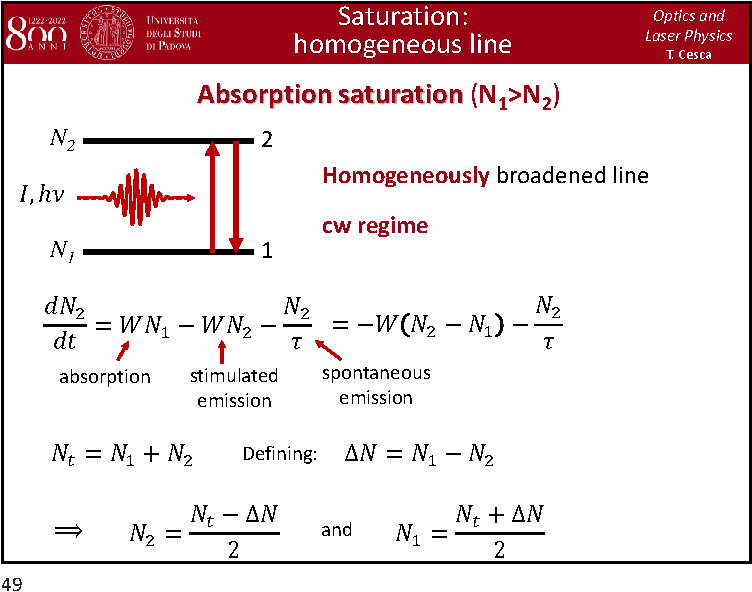
\includegraphics[page=1,width=1\textwidth]{../lessons/pdf_file/10_lecture.pdf}
\end{minipage}
\hspace{0.3cm}\vspace{0.3cm}
\begin{minipage}[c]{0.47\linewidth}

Let us consider a two-level system. We shine with a beam of sufficiently intensity on a material.
If \( N_1 > N_2 \), the material become trasparent to incoming radiation.
\textbf{Absorption saturation}: phenomenon of saturation in absorption.

We suppose an \textbf{homogeneous broadened line} (all atoms in the material can be treated as equal) and we study the process in \textbf{continous wave regime} (we shine continuously).

Let us write the rate equation for the energy level 2: we have absorption (\( W N_1 \)), we have stimulated emission \( -W N_2 \) and spontaneous emission \( - N_2/\tau  \). We are dealing in with non degenerate levels so \( W_{abs} = W_{se} \).

We rewrite the population in the two levels.

\end{minipage}

\subsubsection*{Slide 2}

\begin{minipage}[]{0.5\linewidth}
\centering
\includegraphics[page=2,width=1\textwidth]{../lessons/pdf_file/10_lecture.pdf}
\end{minipage}
\hspace{0.3cm}\vspace{0.3cm}
\begin{minipage}[c]{0.47\linewidth}

We rewrite the rate equation in terms of the different in population. Firstly, we want to obtain a \textbf{steady-state} solution.

We have introduced the \textbf{satuarion intensity}: ration between the energy of the photons that we are shining in the material divided by 2 times the cross section for absorption and the total lifetime (to take into account spontaneous emission process) of the upper energy level.

When the intensity of the beam is equal to the saturation intensity \( I = I_s \), we obtain a difference between the two population which is half the total population.

\end{minipage}

\subsubsection*{Slide 3}

\begin{minipage}[]{0.5\linewidth}
\centering
\includegraphics[page=3,width=1\textwidth]{../lessons/pdf_file/10_lecture.pdf}
\end{minipage}
\hspace{0.3cm}\vspace{0.3cm}
\begin{minipage}[c]{0.47\linewidth}

If we remember the definition of the \textbf{absorption coefficient} \( \alpha  \), we can rewrite it as a function of the saturation intensity. The \( \alpha _0 \) is the \textbf{unsaturated absorption coefficient}: absorption coefficient of the material when the intensity of the beam is close to zero and we are far away from the saturation condition.

\end{minipage}

\newpage

\subsubsection*{Slide 4}

\begin{minipage}[]{0.5\linewidth}
\centering
\includegraphics[page=4,width=1\textwidth]{../lessons/pdf_file/10_lecture.pdf}
\end{minipage}
\hspace{0.3cm}\vspace{0.3cm}
\begin{minipage}[c]{0.47\linewidth}

Let us describe the very same process in a \textbf{pulsed regime} \( I = I (t) \).

We have to distinguish:
\begin{itemize}
\item the case in which the pulse duration is \textbf{much larger} than the upper level lifetime;

\item pulse duration is \textbf{much smaller} than the upper level lifetime.
\end{itemize}


\end{minipage}

\subsubsection*{Slide 5}

\begin{minipage}[]{0.5\linewidth}
\centering
\includegraphics[page=5,width=1\textwidth]{../lessons/pdf_file/10_lecture.pdf}
\end{minipage}
\hspace{0.3cm}\vspace{0.3cm}
\begin{minipage}[c]{0.47\linewidth}

In the first case, if the pulse is so slow, the temporal evolution of \( \Delta N \) is very slow. We can neglect this term in the rate equation.

At the \textbf{steady-state}, the solution of the rate equation is the same for the \textbf{cw} (continuity wave) condition.
We will get the very same expression for the absorption coefficient.

\end{minipage}

\subsubsection*{Slide 6}

\begin{minipage}[]{0.5\linewidth}
\centering
\includegraphics[page=6,width=1\textwidth]{../lessons/pdf_file/10_lecture.pdf}
\end{minipage}
\hspace{0.3cm}\vspace{0.3cm}
\begin{minipage}[c]{0.47\linewidth}

In the second case, by considering the rate equation, the stimulated emission term dominates over the spontaneous emission one and we can neglect it in the rate equation.

\end{minipage}

\newpage

\subsubsection*{Slide 7}

\begin{minipage}[]{0.5\linewidth}
\centering
\includegraphics[page=7,width=1\textwidth]{../lessons/pdf_file/10_lecture.pdf}
\end{minipage}
\hspace{0.3cm}\vspace{0.3cm}
\begin{minipage}[c]{0.47\linewidth}

By replacing the expression of \( W \) and writing explicitly the time dependence of the intensity, we integrate both term with the initial conditions.

\end{minipage}

\subsubsection*{Slide 8}

\begin{minipage}[]{0.5\linewidth}
\centering
\includegraphics[page=8,width=1\textwidth]{../lessons/pdf_file/10_lecture.pdf}
\end{minipage}
\hspace{0.3cm}\vspace{0.3cm}
\begin{minipage}[c]{0.47\linewidth}

The integral of the intensity over the time is called \textbf{fluence}.
In the same way, we can introduce the \textbf{saturation fluence}.

\end{minipage}

\subsubsection*{Slide 9}

\begin{minipage}[]{0.5\linewidth}
\centering
\includegraphics[page=9,width=1\textwidth]{../lessons/pdf_file/10_lecture.pdf}
\end{minipage}
\hspace{0.3cm}\vspace{0.3cm}
\begin{minipage}[c]{0.47\linewidth}

When \( t \rightarrow \infty  \), the fluence has to be replaced with the \textbf{total fluence} \( \Gamma _t \).

\end{minipage}

\subsubsection*{Slide 10}

\begin{minipage}[]{0.5\linewidth}
\centering
\includegraphics[page=10,width=1\textwidth]{../lessons/pdf_file/10_lecture.pdf}
\end{minipage}
\hspace{0.3cm}\vspace{0.3cm}
\begin{minipage}[c]{0.47\linewidth}

We can rewrite the same things in terms of \textbf{absorption coefficient}.

\end{minipage}

\subsubsection*{Slide 11}

\begin{minipage}[]{0.5\linewidth}
\centering
\includegraphics[page=11,width=1\textwidth]{../lessons/pdf_file/10_lecture.pdf}
\end{minipage}
\hspace{0.3cm}\vspace{0.3cm}
\begin{minipage}[c]{0.47\linewidth}

Let us consider the case \( N_1 < N_2 \) (\textbf{gain condition}).
In order to get gain, our material should be in out-of-equilibrium condition.
A \textbf{four-level system} is the most efficient way to get population inversion: we can consider that always \( N_1 \sim 0 \).
We suppose also \textbf{homogeneous broadened line} and \textbf{cw regime}.

The rate equation can be written as a function of the \textbf{pumping rate}, then we have the \emph{stimulated emission} term and \emph{spontaneous emission} term.

Since \( N_1 \sim 0 \), \( N_2 \) is already the population inversion (the difference population wrt the lower level). We find the solution in the \textbf{steady-state}. \( N_{20}  \) is the pumping rate for the total lifetime of the upper laser level.

We introduce also in this case \textbf{saturation intensity}. The saturation intensity depends intrinsically on the property of the material and on the light you are shining.


\end{minipage}

\subsubsection*{Slide 12}

\begin{minipage}[]{0.5\linewidth}
\centering
\includegraphics[page=12,width=1\textwidth]{../lessons/pdf_file/10_lecture.pdf}
\end{minipage}
\hspace{0.3cm}\vspace{0.3cm}
\begin{minipage}[c]{0.47\linewidth}

We write the \textbf{gain coefficient} as a function of the saturation intensity. We have that \( g_0 \) is the \textbf{unsaturated gain coefficient}: if intensity \( I \) is much smaller than \( I_s \) we have that \( g \) is closer to the unsaturated value, on the other hand \( I \ll I_s \) the gain coefficient goes to zero.

\end{minipage}

\subsubsection*{Slide 13}

\begin{minipage}[]{0.5\linewidth}
\centering
\includegraphics[page=13,width=1\textwidth]{../lessons/pdf_file/10_lecture.pdf}
\end{minipage}
\hspace{0.3cm}\vspace{0.3cm}
\begin{minipage}[c]{0.47\linewidth}

Now, let us consider a \textbf{pulsed regime} \( I = I(t) \).

Let us consider the first case in which the pulse duration is much greater than the lifetime of the energy level.
Again, the gain coefficient is the same of the cw regime.

\end{minipage}

\subsubsection*{Slide 14}

\begin{minipage}[]{0.5\linewidth}
\centering
\includegraphics[page=14,width=1\textwidth]{../lessons/pdf_file/10_lecture.pdf}
\end{minipage}
\hspace{0.3cm}\vspace{0.3cm}
\begin{minipage}[c]{0.47\linewidth}

The situation changes when we have the pulse duration much smaller than the lifetime of the upper energy level. The variation over time of \( N_2 \) is dominated by the stimulated emission process.

\end{minipage}

\subsubsection*{Slide 15}

\begin{minipage}[]{0.5\linewidth}
\centering
\includegraphics[page=15,width=1\textwidth]{../lessons/pdf_file/10_lecture.pdf}
\end{minipage}
\hspace{0.3cm}\vspace{0.3cm}
\begin{minipage}[c]{0.47\linewidth}

Again we introduce the \textbf{fluence} and the \textbf{saturation fluence}.

\end{minipage}

\subsubsection*{Slide 16}

\begin{minipage}[]{0.5\linewidth}
\centering
\includegraphics[page=16,width=1\textwidth]{../lessons/pdf_file/10_lecture.pdf}
\end{minipage}
\hspace{0.3cm}\vspace{0.3cm}
\begin{minipage}[c]{0.47\linewidth}

Let us recap what we have seen.

The point to stress is the difference between the \textbf{saturation intensity for absorption} and the \textbf{saturation intensity in the gain condition}. The absorption one is half the value of the gain condition: it means that you can more easily get into a saturation when you are considering absorption wrt gain condition.

\end{minipage}

Let us understand this from a phenomenological point of view:

\begin{itemize}
\item For absorption, we were describing the material as a 2-level system. Any time an absorption transition happen, both the population in the lower and upper energy levels change.

\item On the other hand, for gain, we are considering a 4-level system. The pupulation of the lower laser level is always null. Any time pumping occur, the population of the lower energy level does not change.
\end{itemize}
So, it is much faster to get into saturation for absorption, because any time the two levels that are involved are always affected by the transition and you reach saturation much faster. Indeed, the saturation intensity is smaller.

\subsubsection*{Slide 17}

\begin{minipage}[]{0.5\linewidth}
\centering
\includegraphics[page=17,width=1\textwidth]{../lessons/pdf_file/10_lecture.pdf}
\includegraphics[page=18,width=1\textwidth]{../lessons/pdf_file/10_lecture.pdf}
\end{minipage}
\hspace{0.3cm}\vspace{0.3cm}
\begin{minipage}[c]{0.47\linewidth}

Until now, both for absorption and gain, one of the main assumption is homogeneous broadened line. Let us consider \textbf{inhomogeneous line} (doppler).
We have seen that we have a Gaussian lineshape that we can consider as a convolution of Lorentzian for a set of homogeneously broadened lines.

Let us consider a pump and probe experiment. We are shining a pump beam with intensity \( I(\nu ) \) such that we are able to increase it. At the same time, we scan with a probe with much lower intensity \( I (\nu') \) at different frequency to measure the absorption or the gain coefficient.

\end{minipage}

In this case, if the pump beam reach an intensity so high such that the material goes in saturation, we will observe a \textbf{hole} in the spectrum which correspond to the frequency of the pump beam. The formation of a hole is related to the saturation for homogeneous broadened line, only for that line that is below the gaussian lineshape at the frquency of the pump beam. This is called \textbf{spectral hole burning}.

So, for an \emph{homogeneous broadened line}, when you start saturation you would have a reduction of the intensity without any difference for the difference frequencies.
On the other hand, if you have an \emph{inhomogeneous broadened line} and you perform a pump and probe experiment, you may have saturation only for the homogeneously broadened line centered at the frequency \( \nu  \) of the pump beam and holes in the spectrum are created.



\end{document}
